\section{Parallelization using the CPU}

% -------------------------------------------------------------------------------------- %

\subsection{CPU Architechture}

When referring to CPU architecture one typically either means 
\emph{instruction set architecture (ISA)} when referring to a range of CPUs, or the 
\emph{microarchitechture} of a specific CPU model. The ISA is the blueprint for a set of 
abstract characteristics such as supported instructions, data types, register count, etc. 
The microarchitechture is the \emph{implementation} of this blueprint for a CPU. We 
restrict to the discussion of the microarchitecture for the Intel 3rd gen (Ivy Lake) 
line of processors, though the level of detail is low enough that the statements will 
apply to most modern CPUs built on the x86 64-bit ISA. \\

A processor microarchitecture can be further split to 3 components: 

\begin{itemize}
    \item The front end, which consists of instruction cache and instruction fetch / decode 
    units. This is responsible for fetching batches of instructions from memory, storing 
    the batches in the instruction cache, and decoding the instructions into a set of 
    \emph{micro-operations, or $\mu$Ops}.
    \item The back end (or execution engine), which includes the reorder buffer, 
    unified scheduler (also called reservation station), and various execution ports. 
    Since not all instructions are necessarily dependent on one-another, they often be 
    reordered, or multiple instructions can be executed simultaneously. This is known as 
    \emph{out-of-order execution}. The reorder buffer stores the the \emph{order} of 
    $\mu$Ops until they are retired. The scheduler takes $\mu$Ops and dispatches them to 
    the various ports, each of which is specialized for a subset of instructions. 
    \item The memory system. This includes (typically) three cache levels: L1, L2, and L3.
    The L1 cache is faster than L2, but has a lower storage capacity. The same holds for 
    L2 vs L3 cache.
\end{itemize}

\begin{figure}[ht]
    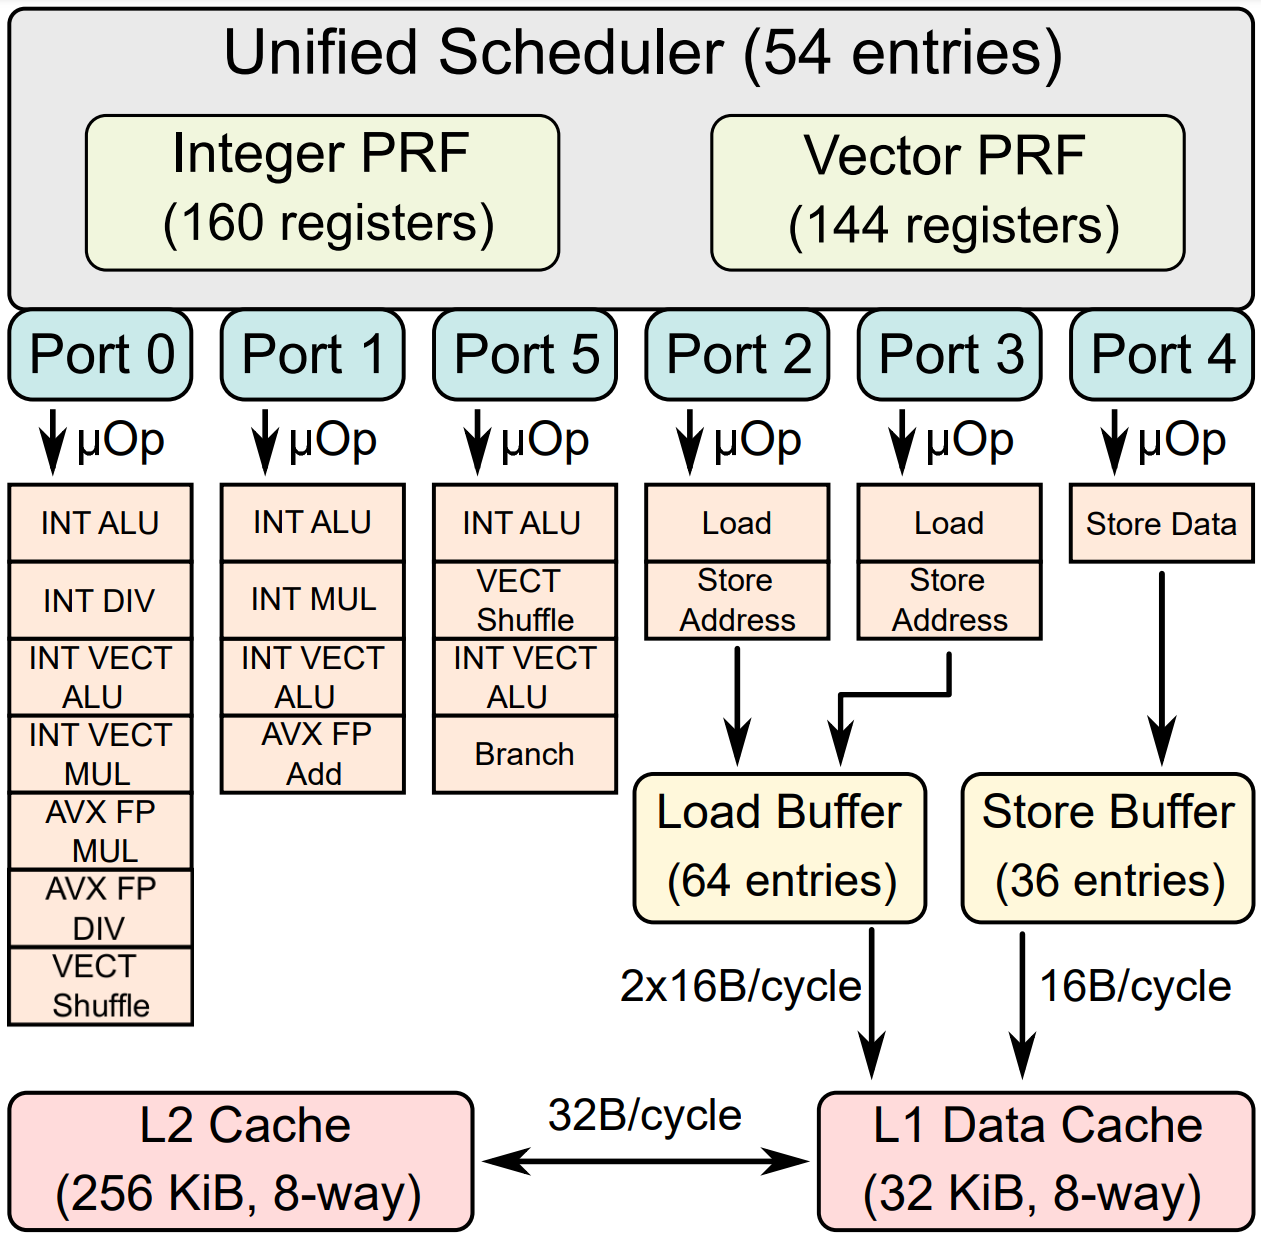
\includegraphics[width=0.6\textwidth]{CPU.png}
    \centering
    \caption{\cite*{solvercomp} Back end for the Intel Ivy Bridge architecture.}
    \label{fig:CPU}
\end{figure}

All three can be limiting factors in a computation, though we will mainly consider 
optimizations for the back end. Additionally, a modern processor will copy this basic 
structure multiple times, each copy is referred to as a \emph{thread}. \\

The naivest but most practically difficult technique to increase performance is to utilize 
the whole instruction set available in the acrhitecture. Obviously it can't be expected 
that the programmer optimizes for every microarchitecture and every instruction; if that were 
true we would all be writing pure assembly language. But there are some easy changes one 
can make, primarily using \emph{fused-multiply-add (FMA)} instructions. An example from 
\cite*{solvercomp}: consider the simple dynamical system over $\mathbb{R}$:

\begin{equation}{}
    x_{k+1} = x_k^2 + p
\end{equation}

for some $p$. To perform one iteration, the CPU needs to call \texttt{MUL} once and then 
\texttt{ADD} once, both of which have latency of roughly 5 clock cycles. Using 
\texttt{FMA}, this can be performed in one operation, nearly doubling performance. A 
consequence of this is that code which does not harness FMA instructions can harness at 
most half of the peak theoretical power of the CPU. \\

In julia, this can be performed with the \jlinl{@muladd} macro from \texttt{MuladdMacro.jl} 
\cite*{muladd}, which automatically converts all combinations of multiply and add into 
calls to the inbuilt \jlinl{muladd} function. \\

Conversely, a conceptually difficult but practically easy technique to implement is 
multithreading. Multithreading is more conceptually difficult because the process of 
creating, scheduling and synchronizing processes over multiple cores is relatively 
complicated. However, due to the obvious benefit offered by multithreaded programming, 
mature libraries have developed to hide these complications under a layer of abstraction. 
In julia, examples include the \jlinl{Threads} module from julia base, as well as the 
package \jlinl{Transducers.jl} \cite*{transducers} which offers a backend for packages 
such as \jlinl{FLoops.jl} \cite*{floops}. Both options offer macros - 
\jlinl{@threads} and \jlinl{@floop} respectively - which can simply be appended to 
\jlinl{for} loops to automatically execute them over multiple threads. \\

Our main technique for parallelization on the CPU is the 
\emph{Advanced Vector eXtension (AVX)}. The philosophy of AVX was initially characterized 
in \cite*{simd} as \emph{Single Instruction Multiple Data (SIMD)}. As the name would 
suggest: when a single instruction, eg. \texttt{ADD}, needs to be applied to multiple 
floating point numbers, then one could pack 4 double precision or 8 single precision 
floating point numbers into a single \emph{vector} stored into the YMM (vector) register. 
This ic alled a \emph{gather} operation.
Two of these vectors can then be passed into port 1 to the AVX floating point 
arithmetic-logic-unit (\texttt{AVX FP ADD} in \autoref{fig:CPU}), and added all at once. 
This reduces the execution time from 20 clock cycles (4 double precision add operations at 
5 clock cycles each) to just 5 clock cycles (1 packed add operation at 5 clock cycles). \\

The majority of modern compilers can automatically convert simple loops and vectorized 
functions into SIMD instructions. This however is not gauranteed, as the compiler neeeds 
to first prove that there are no data dependencies. Hence to reach peak CPU performance, 
it is often required to manually vectorize. 

% -------------------------------------------------------------------------------------- %

\subsection{Implementation in GAIO.jl}

We wish to map an array of test points 
$x = (x_1,\ x_2,\ \ldots,\ x_n),\,\ x_i \in \mathbb{R}^d$ forward, with as much 
parallelism as possible. For example, consider for $d=3$ and a box $[0,1]^3$ the test 
points:

\begin{jllisting}[language=julia, style=jlcodestyle]
    x = [   # each tuple is seen as a point in 3d space
        (1., 0., 0.),
        (0., 1., 0.),
        (0., 0., 1.),
        (0., 0., 0.)
        # etc ...
    ]
\end{jllisting}

We could equivalently characterize this array as an array of packed floats in 
the "packed" space $(\mathbb{R}^4)^3$:

\begin{jllisting}[language=julia, style=jlcodestyle]
    x = [   # three 4xFloat64<...> are seen as a point in our "packed" 3d space
        (
            4xFloat64<1., 0., 0., 0.>, 
            4xFloat64<0., 1., 0., 0.>, 
            4xFloat64<0., 0., 1., 0.>
        )
        # etc ...
    ]
\end{jllisting}

The packed SIMD vectors can be constructed using the \jlinl{Vec} type from \jlinl{SIMD.jl} 
\cite*{simd.jl}, a convenience wrapper around julia's base SIMD vector type (which itself 
is just special tuple). So our goal becomes managing memory careully to (efficiently) 
convert from one vector of vectors to a vector of packed vectors, and vice versa. \\

A convenient fact about the \jlinl{Tuple} type in julia is that if its elements are 
"bits" types (that is, they can be represented by a string of bits that can be \emph{stack-allocated}), 
then the tuple is stored \emph{contiguously} in memory. For eg. numeric types like 
\jlinl{Float32}, this means that the exact positions in memory of each element can be 
deduced from the memory positions of the tuple. Julia provides the convenience function 
\jlinl{reinterpret} which changes the type interpretation of a block of memory. \\

\begin{figure}[ht]
    \ctikzfig{reinterpret}
    \caption{Illustration of julia's \texttt{reinterpret} function, where each square is 1 byte}
    \label{fig:reinterpret}
\end{figure}

Using \jlinl{reinterpret}, we can change the problem to reordering the indices of $x$. 
Hence consider the vector $i$ of indices of $x$: 

\begin{equation}
    i = (\ 
        \underbrace{1,\ 2,\ 3,}_{\text{first point}}\quad 
        \underbrace{4,\ 5,\ 6,}_{\text{second point}}\ 
        \ldots,\ 
        \underbrace{3n-2,\ 3n-1,\ 3n}_{\text{nth point}}
    \ )
\end{equation}

We wish to permute $i$ such that each group of four points has its respective elements 
stored contiguously. Once this is done, we can call \jlinl{reinterpret} again to convert 
the type representation to a vector of packed tuples. In particular we therefore require 
that the number of points $n$ is divisible by $4$. 

\begin{equation}
    S(i) = (\ \underbrace{
        \underbrace{1,\ 4,\ 7,\ 10,}_{\text{first elements}}\quad 
        \underbrace{2,\ 5,\ 8,\ 11,}_{\text{second elements}}\quad
        \underbrace{3,\ 6,\ 9,\ 12,}_{\text{third elements}}\  
    }_{
        \text{first packed point}
    }
        \ldots,\ 
        3n-6,\ 3n-3,\ 3n
    \ )
\end{equation}

We generalize this permutation $S$ to arbitrary dimension $d$, SIMD vector length $s$ and 
vector of points $x$ with length $n$ in \autoref{lst:tuple_vgather}. \\

\begin{jllisting}[float, language=julia, style=jlcodestyle, label=lst:tuple_vgather, caption=Conversion function to packed tuples]
    function tuple_vgather(x::Vector{NTuple{d,T}}, s) where {d,T}
        # x is a vector of tuples, each of length d and datatype T
    
        n = length(x)                                   
        m = n ÷ s
        if n != m * s
            throw(DimensionMismatch("length of input not divisible by simd"))
        end
    
        # Change type interpretation of x's memory
        vr = reinterpret(T, x)
    
        # Initialize the vector of packed tuples
        vo = Vector{NTuple{d,Vec{s,T}}}(undef, m)
    
        # The indices that form the first element of the first packed vector
        idx = Vec(ntuple( i -> (i-1) * d, s ))
    
        # Grab the indices of the first element of the i-th packed vector, 
        # then jump by d*s to grab the indices of the second element, and so on
        for i in 1:m
            vo[i] = ntuple( j -> vr[idx + (i-1) * d * s + j], d )
        end                                             
        
        return vo
    end
\end{jllisting}

This function provides the fundamental technique for parallelization on the CPU. We first 
gather the points, then pass the gathered points to the function $f$. However, we still 
need to convert the packed mapped points back to single points for use with other 
functions afterward. This is the inverse of a gather operation, and is called 
\emph{scatter} (see \autoref{lst:tuple_vscatter}). \\

\begin{jllisting}[float, language=julia, style=jlcodestyle, label=lst:tuple_vscatter, caption=Conversion back to single tuples]
    function tuple_vscatter(y::Vector{NTuple{d,Vec{s,T}}}) where {s,d,T}
        # y is a vector of packed tuples, tuples of SIMD Vecs

        # Initialize the unpacked vector
        vo = Vector{NTuple{d,T}}(undef, s * length(y))

        # Create a view of vo which is made of individual numbers of type T 
        vr = reinterpret(T, vo)

        # The indices that form the first element of the first packed vector
        idx = Vec(ntuple( i -> d * (i-1), s ))

        # set the values of vr as the permuted values of y
        for i in 1:d, j in 1:length(vi)
            vr[idx + (j-1) * d * s + i] = y[i + (j-1) * d]
        end

        return vo
    end
\end{jllisting}

It is important to note that not all elementary instructions have SIMD equivalents. Hence 
some more complicated functions cannot be parallelized in this way. 

% -------------------------------------------------------------------------------------- %

\subsection{Results}



% -------------------------------------------------------------------------------------- %
